\begin{figure}[H]
  \centering
  \textbf{Varying cost }
  \newline
  \newline
  \pgfplotsset{
    scale only axis,
    legend style={at={(0,0.8)}, anchor=west, font=\tiny},
    xmin=15,
  }
  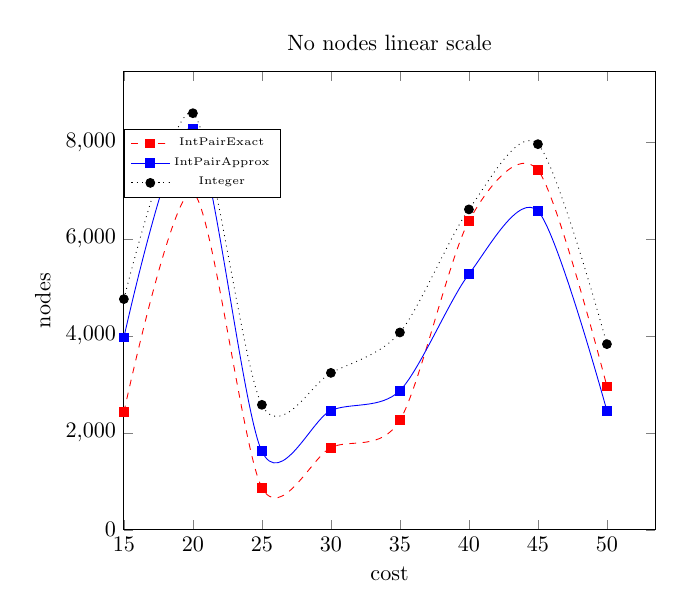
\begin{tikzpicture} [scale=0.8]
    \begin{axis}[
        title=No nodes linear scale,
        ylabel=nodes,
        xtick=data,
        ymin=0, 
        xlabel=cost ]
      \addplot[smooth,mark=square*, mark options={solid},red, dashed]
      coordinates{ (15, 2428) (20, 6960) (25, 872) (30, 1696) (35, 2261) (40, 6373) (45, 7422) (50, 2959)
      }; \label{ie_plot} \addlegendentry{IntPairExact}
      \addplot[smooth,mark=square*, mark options={solid},blue]
      coordinates{ (15, 3969) (20, 8278) (25, 1619) (30, 2461) (35, 2873) (40, 5276) (45, 6577) (50, 2455)
      }; \label{ia_plot} \addlegendentry{IntPairApprox}
      \addplot[smooth,mark=*,mark options={solid},black, dotted]
      coordinates{ (15, 4760) (20, 8596) (25, 2579) (30, 3238) (35, 4072) (40, 6611) (45, 7957) (50, 3831)
      }; \label{int_plot} \addlegendentry{Integer}
    \end{axis}
  \end{tikzpicture}
  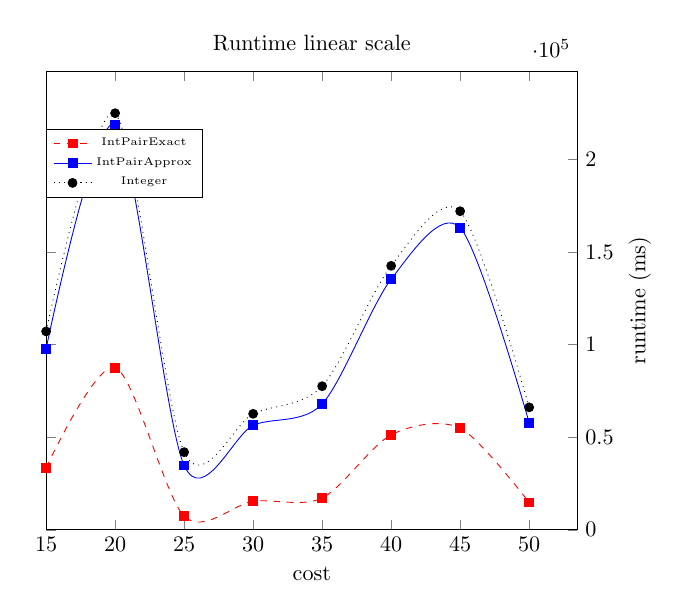
\begin{tikzpicture} [scale=0.8]
    \begin{axis}[
        yticklabel pos=right,
        xtick=data,
        title=Runtime linear scale,
        ylabel=runtime (ms),
        xlabel=cost,
        ymin=0, ]
      \addplot[smooth,mark=square*,mark options={solid},red, dashed]
      coordinates{ (15,33465) (20,87636) (25,7373) (30,15440) (35,17133) (40,51271) (45,54898) (50,14749)
      }; \label{IntPairExact Run}
      \addplot[smooth,mark=square*,mark options={solid},blue]
      coordinates{ (15,97813) (20,218750) (25,34761) (30,56398) (35,67953) (40,135341) (45,163128) (50,57833)
      }; \label{IntPairApprox Run}
      \addplot[smooth,mark=*,mark options={solid},black, dotted]
      coordinates{ (15,107122) (20,224958) (25,41936) (30,62636) (35,77550) (40,142552) (45,172028) (50,66124)
      }; \label{IntegerRun}
      \addlegendentry{IntPairExact}
      \addlegendentry{IntPairApprox}
      \addlegendentry{Integer}
    \end{axis}
  \end{tikzpicture}

  
\begin{tikzpicture}[scale=1.4]
    \draw[very thick] (-4,0) -- (4,0);
    \draw[draw=white] (-5,-0.2) -- (5,-0.2);
  \end{tikzpicture}


  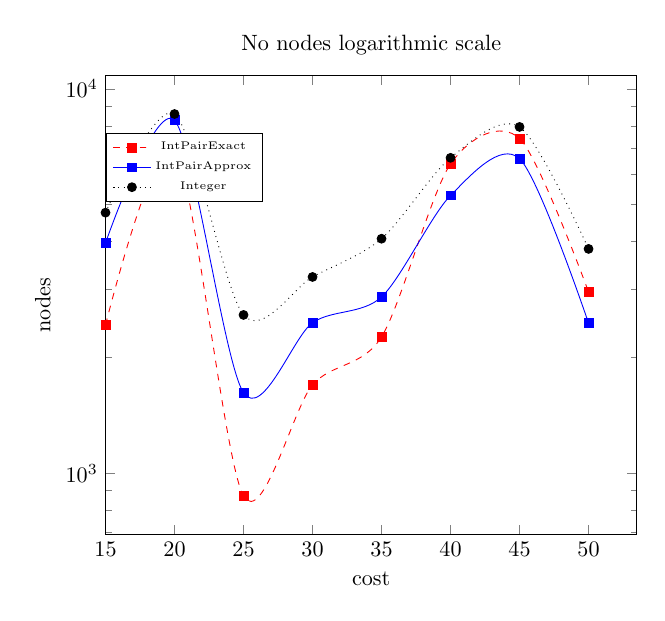
\begin{tikzpicture} [scale=0.8]
    \begin{semilogyaxis}[
        title=No nodes logarithmic scale,
        ylabel=nodes,
        xtick=data,
        ymin=0, 
        xlabel=cost ]
     \addplot[smooth,mark=square*, mark options={solid},red, dashed]
      coordinates{ (15, 2428) (20, 6960) (25, 872) (30, 1696) (35, 2261) (40, 6373) (45, 7422) (50, 2959)
      }; \label{ie_plot} \addlegendentry{IntPairExact}
      \addplot[smooth,mark=square*, mark options={solid},blue]
      coordinates{ (15, 3969) (20, 8278) (25, 1619) (30, 2461) (35, 2873) (40, 5276) (45, 6577) (50, 2455)
      }; \label{ia_plot} \addlegendentry{IntPairApprox}
      \addplot[smooth,mark=*,mark options={solid},black, dotted]
      coordinates{ (15, 4760) (20, 8596) (25, 2579) (30, 3238) (35, 4072) (40, 6611) (45, 7957) (50, 3831)
      }; \label{int_plot} \addlegendentry{Integer}

    \end{semilogyaxis}
  \end{tikzpicture}
  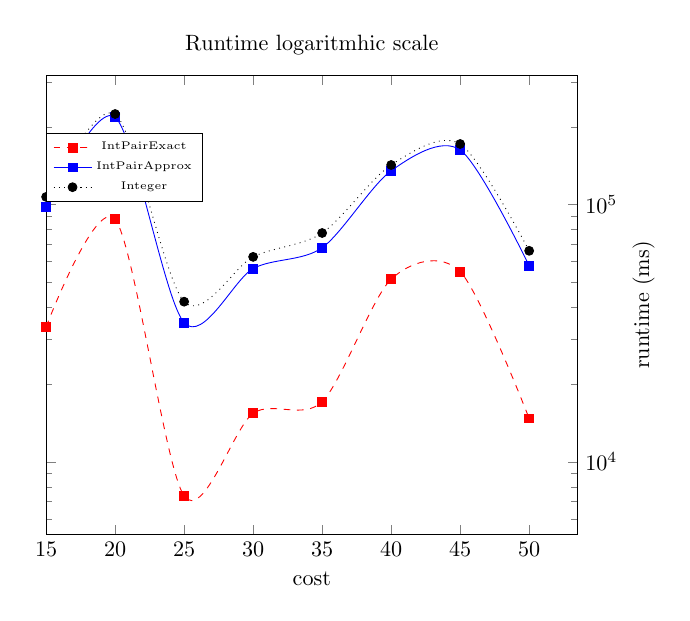
\begin{tikzpicture} [scale=0.8]
    \begin{semilogyaxis}[
        title=Runtime logaritmhic scale,
        yticklabel pos=right,
        xtick=data,
        ylabel=runtime (ms),
        xlabel=cost,
        ymin=0,  ]
      \addplot[smooth,mark=square*,mark options={solid},red, dashed]
      coordinates{ (15,33465) (20,87636) (25,7373) (30,15440) (35,17133) (40,51271) (45,54898) (50,14749)
      }; \label{IntPairExact Run}
      \addplot[smooth,mark=square*,mark options={solid},blue]
      coordinates{ (15,97813) (20,218750) (25,34761) (30,56398) (35,67953) (40,135341) (45,163128) (50,57833)
      }; \label{IntPairApprox Run}
      \addplot[smooth,mark=*,mark options={solid},black, dotted]
      coordinates{ (15,107122) (20,224958) (25,41936) (30,62636) (35,77550) (40,142552) (45,172028) (50,66124)
      }; \label{IntegerRun}
      \addlegendentry{IntPairExact}
      \addlegendentry{IntPairApprox}
      \addlegendentry{Integer}
    \end{semilogyaxis}
  \end{tikzpicture}
  \caption{{Caption}}\label{fig:}
\end{figure}
